\documentclass[11pt,letterpaper]{article}
\usepackage[lmargin=1in,rmargin=1in,tmargin=1in,bmargin=1in]{geometry}
\usepackage{../style/homework}
\usepackage{../style/commands}
\setbool{quotetype}{true} % True: Side; False: Under
\setbool{hideans}{false} % Student: True; Instructor: False

% -------------------
% Content
% -------------------
\begin{document}

\homework{10: Due 11/08}{Thankfully, perseverance is a great substitute for talent.}{Steve Martin}

% Problem 1
\problem{10} Factor $x^2 + 2x - 24$. Show all your work. \pspace

\sol 
	\begin{table}[!ht]
	\centering
	\underline{\bfseries 24} \pvspace{0.2cm}
	\begin{tabular}{rr}
	$1 \cdot -24 \colon$ & $-23$ \\
	$-1 \cdot 24 \colon$ & $23$ \\
	$2 \cdot -12 \colon$ & $-10$ \\
	$-2 \cdot 12 \colon$ & $10$ \\
	$3 \cdot -8 \colon$ & $-5$ \\
	$-3 \cdot 8 \colon$ & $5$ \\
	$4 \cdot -6 \colon$ & $-2$ \\ \hline
	\multicolumn{1}{|r}{$-4 \cdot 6 \colon$} & \multicolumn{1}{r|}{$2$} \\ \hline
	\end{tabular}
	\end{table}

Therefore,
	\[
	x^2 + 2x - 24= (x - 4)(x + 6)
	\]





\newpage





% Problem 2
\problem{10} Factor $x^2 + 4x - 32$. Show all your work. \pspace

\sol 
	\begin{table}[!ht]
	\centering
	\underline{\bfseries 32} \pvspace{0.2cm}
	\begin{tabular}{rr}
	$1 \cdot -32 \colon$ & $-31$ \\
	$-1 \cdot 32 \colon$ & $31$ \\
	$2 \cdot -16 \colon$ & $-14$ \\
	$-2 \cdot 16 \colon$ & $14$ \\
	$4 \cdot -8 \colon$ & $-4$ \\ \hline
	\multicolumn{1}{|r}{$-4 \cdot 8 \colon$} & \multicolumn{1}{r|}{$4$} \\ \hline
	\end{tabular}
	\end{table}

Therefore,
	\[
	x^2 + 4x - 32= (x - 4)(x + 8)
	\]





\newpage





% Problem 3
\problem{10} Factor $x^2 + 4x$. Show all your work. \pspace

\sol This quadratic expression factors as\dots
	\[
	x^2 + 4x= x(x + 4)
	\]





\newpage





% Problem 4
\problem{10} Factor $x^2 + 17x - 18$. Show all your work. \pspace

\sol 
	\begin{table}[!ht]
	\centering
	\underline{\bfseries 18} \pvspace{0.1cm}
	\begin{tabular}{rr}
	$1 \cdot -18 \colon$ & $-17$ \\ \hline
	\multicolumn{1}{|r}{$-1 \cdot 18 \colon$} & \multicolumn{1}{r|}{$17$} \\ \hline
	$2 \cdot -9 \colon$ & $-7$ \\
	$-2 \cdot 9 \colon$ & $7$ \\
	$3 \cdot -6 \colon$ & $-3$ \\
	$-3 \cdot 6 \colon$ & $3$ \\
	\end{tabular}
	\end{table}

Therefore,
	\[
	x^2 + 17x - 18= (x - 1)(x + 18)
	\]




\newpage





% Problem 5
\problem{10} Factor $2x^2 - 11x + 15$. Show all your work. \pspace

\sol 
	\begin{table}[!ht]
	\centering
	\underline{\bfseries 15} \pvspace{0.1cm}
	\begin{tabular}{c}
	$1 \cdot 15$ \\
	$-1 \cdot -15$ \\
	$3 \cdot 5$ \\
	$-3 \cdot -5$
	\end{tabular}
	\end{table}

Then as $2= 1 \cdot 2$, we have\dots
	\[
	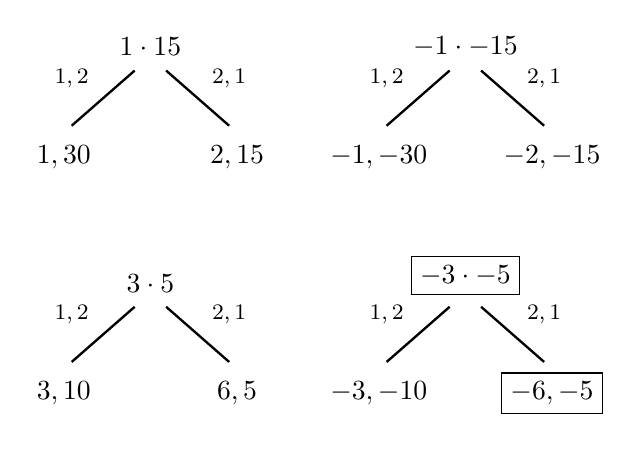
\begin{tikzpicture}
	\node at (0,0) {$1 \cdot 15$};
	\node at (-1.0,-0.4) {\footnotesize$1, 2$};
	\draw[line width=0.03cm,label={1}] (-0.2,-0.3) -- (-1,-1);
	\node at (-1.1,-1.4) {$1, 30$};
	\node at (1.0,-0.4) {\footnotesize$2,1$};
	\draw[line width=0.03cm] (0.2,-0.3) -- (1,-1);
	\node at (1.1,-1.4) {$2, 15$};	
	
	\tikzset{shift={(4,0)}}

	\node at (0,0) {$-1 \cdot -15$};
	\node at (-1.0,-0.4) {\footnotesize$1, 2$};
	\draw[line width=0.03cm,label={1}] (-0.2,-0.3) -- (-1,-1);
	\node at (-1.1,-1.4) {$-1, -30$};
	\node at (1.0,-0.4) {\footnotesize$2,1$};
	\draw[line width=0.03cm] (0.2,-0.3) -- (1,-1);
	\node at (1.1,-1.4) {$-2, -15$};

	\tikzset{shift={(-4,-3)}}

	\node at (0,0) {$3 \cdot 5$};
	\node at (-1.0,-0.4) {\footnotesize$1, 2$};
	\draw[line width=0.03cm,label={1}] (-0.2,-0.3) -- (-1,-1);
	\node at (-1.1,-1.4) {$3, 10$};
	\node at (1.0,-0.4) {\footnotesize$2,1$};
	\draw[line width=0.03cm] (0.2,-0.3) -- (1,-1);
	\node at (1.1,-1.4) {$6, 5$};

	\tikzset{shift={(4,0)}}

	\node at (0,0.1) {\framebox{$-3 \cdot -5$}};
	\node at (-1.0,-0.4) {\footnotesize$1, 2$};
	\draw[line width=0.03cm,label={1}] (-0.2,-0.3) -- (-1,-1);
	\node at (-1.1,-1.4) {$-3, -10$};
	\node at (1.0,-0.4) {\footnotesize$2,1$};
	\draw[line width=0.03cm] (0.2,-0.3) -- (1,-1);
	\node at (1.1,-1.4) {\framebox{$-6, -5$}};
	\end{tikzpicture}
	\]

Therefore, 
	\[
	2x^2 - 11x + 15= (2x - 5)(x - 3)
	\]




\newpage





% Problem 6
\problem{10} Factor $3x^2 + 5x - 2$. Show all your work. \pspace

\sol 
	\begin{table}[!ht]
	\centering
	\underline{\bfseries 2} \pvspace{0.1cm}
	\begin{tabular}{c}
	$1 \cdot -2$ \\
	$-1 \cdot 2$
	\end{tabular}
	\end{table}

Then as $3= 1 \cdot 3$, we have\dots
	\[
	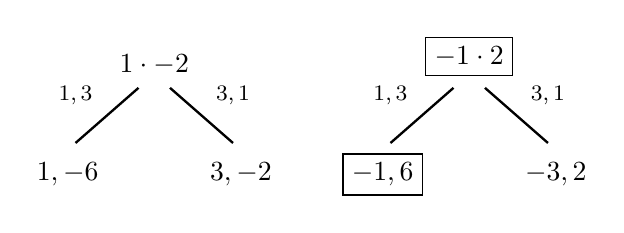
\begin{tikzpicture}
	\node at (0,0) {$1 \cdot -2$};
	\node at (-1.0,-0.4) {\footnotesize$1, 3$};
	\draw[line width=0.03cm,label={1}] (-0.2,-0.3) -- (-1,-1);
	\node at (-1.1,-1.4) {$1, -6$};
	\node at (1.0,-0.4) {\footnotesize$3,1$};
	\draw[line width=0.03cm] (0.2,-0.3) -- (1,-1);
	\node at (1.1,-1.4) {$3, -2$};	
	
	\tikzset{shift={(4,0)}}

	\node at (0,0.1) {\framebox{$-1 \cdot 2$}};
	\node at (-1.0,-0.4) {\footnotesize$1, 3$};
	\draw[line width=0.03cm,label={1}] (-0.2,-0.3) -- (-1,-1);
	\node at (-1.1,-1.4) {\framebox{$-1, 6$}};
	\node at (1.0,-0.4) {\footnotesize$3,1$};
	\draw[line width=0.03cm] (0.2,-0.3) -- (1,-1);
	\node at (1.1,-1.4) {$-3, 2$};
	\end{tikzpicture}
	\]

Therefore, 
	\[
	3x^2 + 5x - 2= (x + 2)(3x - 1)
	\]





\newpage





% Problem 7
\problem{10} Factor $x^2 - 6x + 9$. Show all your work. \pspace

\sol 
	\begin{table}[!ht]
	\centering
	\underline{\bfseries 9} \pvspace{0.1cm}
	\begin{tabular}{rr}
	$1 \cdot 9 \colon$ & $10$ \\
	$-1 \cdot -9 \colon$ & $-10$ \\
	$3 \cdot 3 \colon$ & $6$ \\ \hline
	\multicolumn{1}{|r}{$-3 \cdot -3 \colon$} & \multicolumn{1}{r|}{$-6$} \\ \hline
	\end{tabular}
	\end{table}

Therefore,
	\[
	x^2 - 6x + 9= (x - 3)(x - 3)= (x - 3)^2
	\]





\newpage





% Problem 8
\problem{10} Factor $x^2 + 10x + 16$. Show all your work. \pspace

\sol 
	\begin{table}[!ht]
	\centering
	\underline{\bfseries 16} \pvspace{0.1cm}
	\begin{tabular}{rr}
	$1 \cdot 16 \colon$ & $17$ \\
	$-1 \cdot -16 \colon$ & $-17$ \\ \hline
	\multicolumn{1}{|r}{$2 \cdot 8 \colon$} & \multicolumn{1}{r|}{$10$} \\ \hline
	$-2 \cdot -8 \colon$ & $-10$ \\
	$4 \cdot 4 \colon$ & $8$ \\
	$-4 \cdot -4 \colon$ & $-8$ \\
	\end{tabular}
	\end{table}

Therefore,
	\[
	x^2 + 10x + 16= (x + 2)(x + 8)
	\]





\newpage





% Problem 9
\problem{10} Factor $4x^2 - 4x - 3$. Show all your work. \pspace

\sol
	\begin{table}[!ht]
	\centering
	\underline{\bfseries 3} \pvspace{0.1cm}
	\begin{tabular}{c}
	$1 \cdot -3$ \\
	$-1 \cdot 3$
	\end{tabular}
	\end{table}

Then as $4= 1 \cdot 4$ or $4= 2 \cdot 2$, we have\dots
	\[
	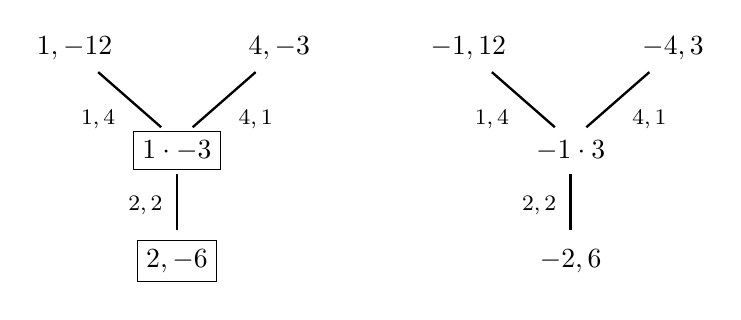
\begin{tikzpicture}
	\node at (0,0) {\framebox{$1 \cdot -3$}};
	\node at (-0.4,-0.7) {\footnotesize$2, 2$};
	\draw[line width=0.03cm,label={1}] (0,-0.3) -- (0,-1);
	\node at (0,-1.4) {\framebox{$2, -6$}};
	\node at (-1,0.4) {\footnotesize$1, 4$};	
	\draw[line width=0.03cm] (-0.2,0.3) -- (-1,1);
	\node at (-1.3,1.3) {$1, -12$};
	\node at (1,0.4) {\footnotesize$4, 1$};
	\draw[line width=0.03cm] (0.2,0.3) -- (1,1);
	\node at (1.3,1.3) {$4, -3$};
	
	\tikzset{shift={(5,0)}}

	\node at (0,0) {$-1 \cdot 3$};
	\node at (-0.4,-0.7) {\footnotesize$2, 2$};
	\draw[line width=0.03cm,label={1}] (0,-0.3) -- (0,-1);
	\node at (0,-1.4) {$-2, 6$};
	\node at (-1,0.4) {\footnotesize$1, 4$};	
	\draw[line width=0.03cm] (-0.2,0.3) -- (-1,1);
	\node at (-1.3,1.3) {$-1, 12$};
	\node at (1,0.4) {\footnotesize$4, 1$};
	\draw[line width=0.03cm] (0.2,0.3) -- (1,1);
	\node at (1.3,1.3) {$-4, 3$};
	\end{tikzpicture}
	\]

Therefore, 
	\[
	4x^2 - 4x - 3= (2x - 3)(2x + 1)
	\]





\newpage





% Problem 10
\problem{10} Factor $12x^2 + 13x - 4$. Show all your work. \pspace

\sol
	\begin{table}[!ht]
	\centering
	\underline{\bfseries 4} \pvspace{0.1cm}
	\begin{tabular}{c}
	$1 \cdot -4$ \\
	$-1 \cdot 4$ \\
	$2 \cdot -2$
	\end{tabular}
	\end{table}

Then as $12= 1 \cdot 12$, $12= 2 \cdot 6$, or $12= 3 \cdot 4$, we have\dots
	\[
	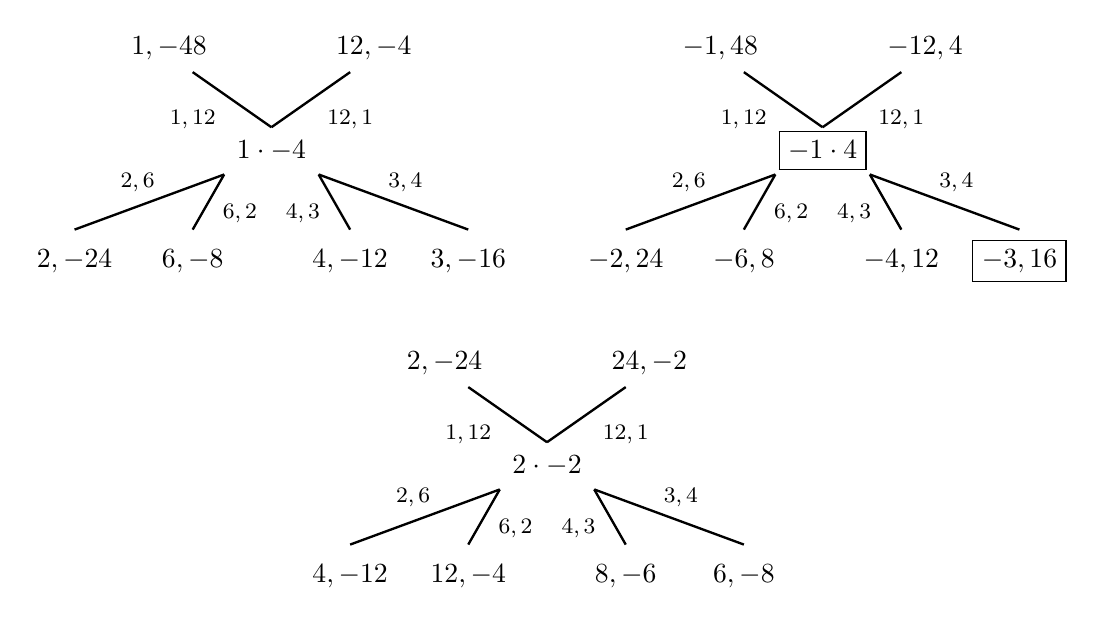
\begin{tikzpicture}
	\node at (0,0) {$1 \cdot -4$};
	
	\node at (-1,0.4) {\footnotesize$1, 12$};	
	\draw[line width=0.03cm] (0,0.3) -- (-1,1);
	\node at (-1.3,1.3) {$1, -48$};
	
	\node at (1,0.4) {\footnotesize$12, 1$};
	\draw[line width=0.03cm] (0,0.3) -- (1,1);
	\node at (1.3,1.3) {$12, -4$};
	
	\node at (-1.7,-0.4) {\footnotesize$2, 6$};
	\draw[line width=0.03cm,label={1}] (-0.6,-0.3) -- (-2.5,-1);
	\node at (-2.5,-1.4) {$2, -24$};
	
	\node at (-0.4,-0.8) {\footnotesize$6, 2$};
	\draw[line width=0.03cm,label={1}] (-0.6,-0.3) -- (-1,-1);
	\node at (-1,-1.4) {$6, -8$};
	
	\node at (1.7,-0.4) {\footnotesize$3, 4$};
	\draw[line width=0.03cm,label={1}] (0.6,-0.3) -- (2.5,-1);
	\node at (2.5,-1.4) {$3, -16$};

	\node at (0.4,-0.8) {\footnotesize$4, 3$};
	\draw[line width=0.03cm,label={1}] (0.6,-0.3) -- (1,-1);
	\node at (1,-1.4) {$4, -12$};
	
	\tikzset{shift={(7,0)}}

	\node at (0,0) {\framebox{$-1 \cdot 4$}};
	
	\node at (-1,0.4) {\footnotesize$1, 12$};	
	\draw[line width=0.03cm] (0,0.3) -- (-1,1);
	\node at (-1.3,1.3) {$-1, 48$};
	
	\node at (1,0.4) {\footnotesize$12, 1$};
	\draw[line width=0.03cm] (0,0.3) -- (1,1);
	\node at (1.3,1.3) {$-12, 4$};
	
	\node at (-1.7,-0.4) {\footnotesize$2, 6$};
	\draw[line width=0.03cm,label={1}] (-0.6,-0.3) -- (-2.5,-1);
	\node at (-2.5,-1.4) {$-2, 24$};
	
	\node at (-0.4,-0.8) {\footnotesize$6, 2$};
	\draw[line width=0.03cm,label={1}] (-0.6,-0.3) -- (-1,-1);
	\node at (-1,-1.4) {$-6, 8$};
	
	\node at (1.7,-0.4) {\footnotesize$3, 4$};
	\draw[line width=0.03cm,label={1}] (0.6,-0.3) -- (2.5,-1);
	\node at (2.5,-1.4) {\framebox{$-3, 16$}};

	\node at (0.4,-0.8) {\footnotesize$4, 3$};
	\draw[line width=0.03cm,label={1}] (0.6,-0.3) -- (1,-1);
	\node at (1,-1.4) {$-4, 12$};

	\tikzset{shift={(-3.5,-4)}}	

	\node at (0,0) {$2 \cdot -2$};
	
	\node at (-1,0.4) {\footnotesize$1, 12$};	
	\draw[line width=0.03cm] (0,0.3) -- (-1,1);
	\node at (-1.3,1.3) {$2, -24$};
	
	\node at (1,0.4) {\footnotesize$12, 1$};
	\draw[line width=0.03cm] (0,0.3) -- (1,1);
	\node at (1.3,1.3) {$24, -2$};
	
	\node at (-1.7,-0.4) {\footnotesize$2, 6$};
	\draw[line width=0.03cm,label={1}] (-0.6,-0.3) -- (-2.5,-1);
	\node at (-2.5,-1.4) {$4, -12$};
	
	\node at (-0.4,-0.8) {\footnotesize$6, 2$};
	\draw[line width=0.03cm,label={1}] (-0.6,-0.3) -- (-1,-1);
	\node at (-1,-1.4) {$12, -4$};
	
	\node at (1.7,-0.4) {\footnotesize$3, 4$};
	\draw[line width=0.03cm,label={1}] (0.6,-0.3) -- (2.5,-1);
	\node at (2.5,-1.4) {$6, -8$};

	\node at (0.4,-0.8) {\footnotesize$4, 3$};
	\draw[line width=0.03cm,label={1}] (0.6,-0.3) -- (1,-1);
	\node at (1,-1.4) {$8, -6$};


	\end{tikzpicture}
	\]

Therefore, 
	\[
	12x^2 + 13x - 4= (3x + 4)(4x - 1)
	\]


%\printpoints
\end{document}